\documentclass[11pt]{beamer}
\usepackage[utf8]{inputenc}
\usepackage[T1]{fontenc}
\usepackage{lmodern}
\usepackage{amsmath}
\usepackage{amsfonts}
\usepackage{amssymb}
\usepackage{graphicx}
\usepackage{tikz}
\usepackage{xspace}
\usepackage{hyperref}
\usepackage{xcolor}
\usetheme{Singapore}

\usepackage{environ}
\makeatletter
\newsavebox{\measure@tikzpicture}
\NewEnviron{scaletikzpicturetowidth}[1]{%
	\def\tikz@width{#1}%
	\def\tikzscale{1}\begin{lrbox}{\measure@tikzpicture}%
		\BODY
	\end{lrbox}%
	\pgfmathparse{#1/\wd\measure@tikzpicture}%
	\edef\tikzscale{\pgfmathresult}%
	\BODY
}

\definecolor{B}{RGB}{200,37,6}
\definecolor{D}{RGB}{3,101,192}

\begin{document}
	\author{Quan Gan}
	\title{Recommender Systems and DGL}
	%\subtitle{}
	%\logo{}
	\institute{AWS Shanghai AI Lab}
	%\date{}
	%\subject{}
	%\setbeamercovered{transparent}
	%\setbeamertemplate{navigation symbols}{}
	\begin{frame}[plain]
		\maketitle
	\end{frame}

	\begin{frame}
		\frametitle{Why Recommendation}
		\only<2>{\begin{center}
			\centering
			\Huge \bf We don't want our customers to think (hard).
		\end{center}}
		\only<3-4>{
			\begin{center}
				\centering
				Good relevant recommendations make the customers adhere to us.
				
				\only<3>{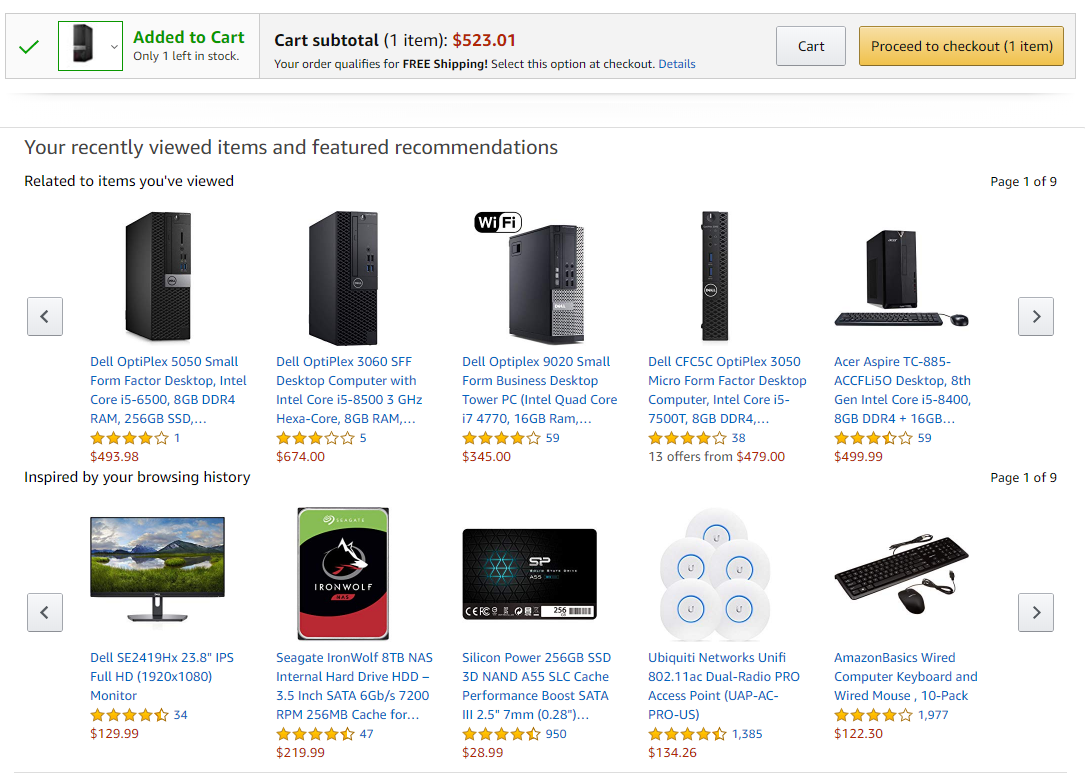
\includegraphics[width=0.8\textwidth]{images/good-recommendation2.png}
				}
				\only<4>{				
\includegraphics[width=0.8\textwidth]{images/good-recommendation.png}}
			\end{center}
		}
	\end{frame}
	
	\begin{frame}
		\frametitle{Recommender System: Problem Statement}
		\begin{center}
			\centering
			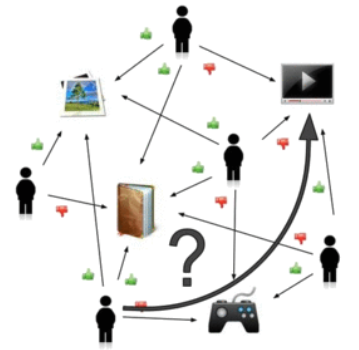
\includegraphics[height=0.7\textheight]{images/cf-stage1.png}
			
			{\tiny Image source: Wikipedia}
		\end{center}
	\end{frame}
	
	\begin{frame}
		\frametitle{Collaborative Filtering}
		\begin{columns}
			\begin{column}{0.3\textwidth}
				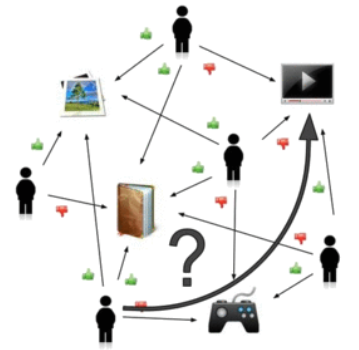
\includegraphics[width=\textwidth]{images/cf-stage1.png}
			\end{column}\pause
			\begin{column}{0.05\textwidth}
				\begin{scaletikzpicturetowidth}{\textwidth}
					\begin{tikzpicture}[scale=\tikzscale]
					\draw [->] (0, 0) -- (0.05, 0);
					\end{tikzpicture}
				\end{scaletikzpicturetowidth}
			\end{column}
			\begin{column}{0.3\textwidth}
				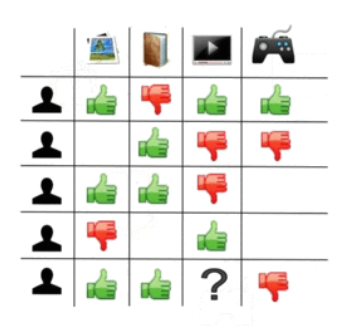
\includegraphics[width=\textwidth]{images/cf-stage2.png}
			\end{column}\pause
			\begin{column}{0.05\textwidth}
				\begin{scaletikzpicturetowidth}{\textwidth}
					\begin{tikzpicture}[scale=\tikzscale]
					\draw [->] (0, 0) -- (0.05, 0);
					\end{tikzpicture}
				\end{scaletikzpicturetowidth}
			\end{column}
			\begin{column}{0.3\textwidth}
				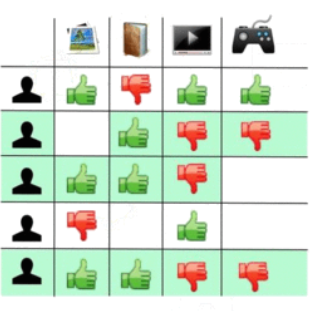
\includegraphics[width=\textwidth]{images/cf-stage3.png}
			\end{column}
		\end{columns}
		\note{Interactions can be inferred by looking at similar users/items.  Users/items are similar if they share some interaction pattern.}
		\begin{center}
			\centering
			{\tiny Image source: Wikipedia}
		\end{center}
	\end{frame}

	\begin{frame}
		\frametitle{Collaborative Filtering: Classical Methods}
		\begin{columns}
			\begin{column}{0.5\textwidth}
				\begin{itemize}
					\item \textbf{User-based}: Infer how a user $i$ would act to an item $j$ by looking at how users that have similar interactions to user $i$ acted to item $j$.
					\begin{itemize}
						\item<2-> We have millions of customers.
						\item<3-> User profiles change constantly and quickly, requiring frequent rebuilds (which are expensive already).
						\item<4-> Not interpretable (can't answer why a user prefers this).
					\end{itemize}
				\end{itemize}
			\end{column}
			\begin{column}{0.5\textwidth}
				\begin{center}
					\centering
					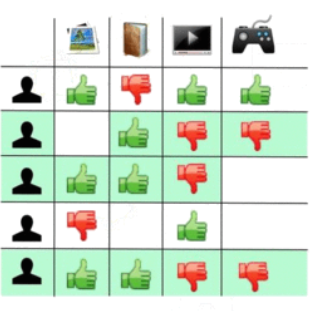
\includegraphics[width=\textwidth]{images/cf-stage3.png}
				\end{center}
			\end{column}
		\end{columns}
	\end{frame}

	\begin{frame}
		\frametitle{Machine Learning Kicks In}
		\begin{columns}
			\begin{column}{0.5\textwidth}
				\begin{center}
					\centering
					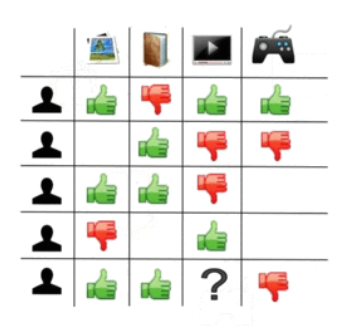
\includegraphics[width=\textwidth]{images/cf-stage2.png}
					
					We were "representing" users and items with the items/users that had interactions with them.
				\end{center}
			\end{column}\pause
			\begin{column}{0.5\textwidth}
				\begin{center}
					\centering
					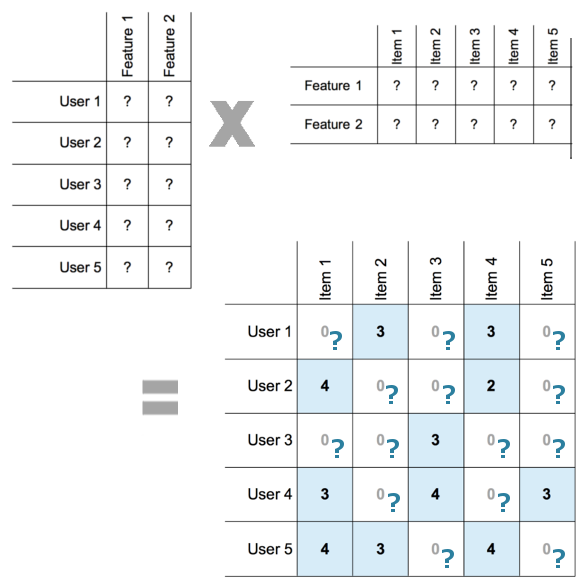
\includegraphics[width=\textwidth]{images/matrix_factorization.png}
					
					{\tiny Source: \href{https://katbailey.github.io/post/matrix-factorization-with-tensorflow/}{\color{blue} Kat Bailey}}
					
					Can we represent users and items as a set of features?
				\end{center}
			\end{column}
		\end{columns}
	\end{frame}

	\begin{frame}
		\frametitle{Latent User/Item Representations}
		\begin{columns}
			\begin{column}{0.6\textwidth}
				\begin{itemize}
					\item<1-> An item can be described with a \only<1-3>{set of features (e.g. how sweet some food is).}%
					\only<4->{\alert<4>{vector $v_j$} (sweet, organic, etc.).}
					\item<2-> A user can be described with \only<1-4>{preferences of the same set of features (e.g. how much a user likes sweet food).}%
					\only<5->{\alert<5>{another vector $u_i$} (likes sweet, likes organic, etc.)}
					\item<3-> The \only<1-5>{interaction}%
					\only<6->{\alert<6>{rating on item $j$ by user $i$}.}
					is defined by \only<1-5>{how well the item features match the user preferences.}%
					\only<6->{\alert<6>{$u_i^\top v_j$}.}
					\item<7-> \alert<7>{We minimize
					$$
					\begin{gathered}
					\sum_{
						\only<1-9>{i,j}\only<10>{\alert{(i, j) \in \mathcal{B}}}
					}\left(r_{i,j} - \left( u_i^\top v_j
					\only<8->{\alert<8>{+ b_{u_i} + b_{v_j}}}\right) \right)^2 \\
					\only<9->{\alert<9>{+ \alpha\mathcal{R}(U, V)}}
					\end{gathered}
					$$}
				\end{itemize}
			\end{column}
			\begin{column}{0.4\textwidth}
				\begin{center}
					\centering
					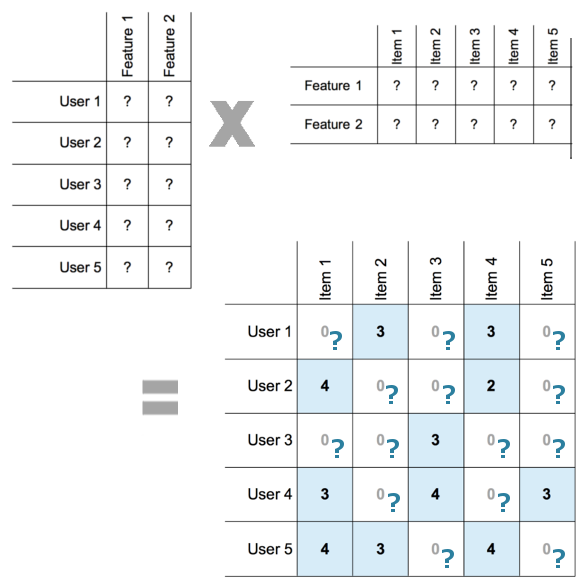
\includegraphics[width=\textwidth]{images/matrix_factorization.png}
					
					{\tiny Source: \href{https://katbailey.github.io/post/matrix-factorization-with-tensorflow/}{\color{blue} Kat Bailey}}
				\end{center}
			\end{column}
		\end{columns}
	\end{frame}

	\begin{frame}
		\frametitle{What if we don't have ratings?}
		\begin{columns}
			\begin{column}{0.5\textwidth}
				\begin{center}
					\centering
					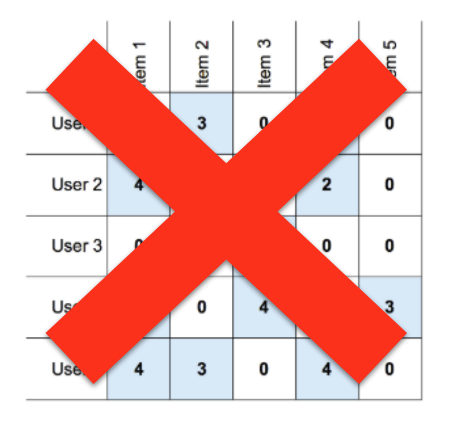
\includegraphics[width=\textwidth]{images/no-rating.png}
				\end{center}
			\end{column}
			\begin{column}{0.5\textwidth}
				\begin{center}
					\centering
					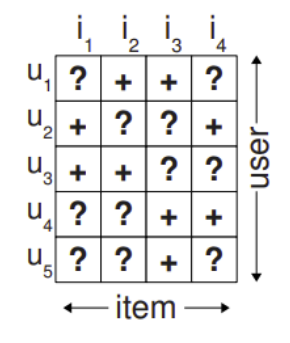
\includegraphics[width=\textwidth]{images/implicit.png}
					
					{\tiny Source: \textit{BPR: Bayesian Personalized Ranking from Implicit Feedback}, Rendle et al. 2012}
				\end{center}
			\end{column}
		\end{columns}
	\end{frame}

	\begin{frame}
		\frametitle{Implicit Feedback}
		\begin{columns}
			\begin{column}{0.6\textwidth}
				\begin{itemize}
					\item<1-> For a given user $i$, an item being interacted $j$ should have a higher score than another item $k$ which was never being interacted.
					\item<2-> We maximize
					$$
					\sum_{i,j,k\in I \backslash I_{u_i}}
					\log \mathrm{sigmoid}(\left(u_i^\top v_j - u_i^\top v_k\right))
					$$
					\item<3-> We usually \emph{sample} one or multiple $k$ when computing gradients (\textbf{negative sampling}).
					\begin{itemize}
						\item Commonly uniformly, but adaptive sampling often helps.
					\end{itemize}
				\end{itemize}
			\end{column}
			\begin{column}{0.4\textwidth}
				\begin{center}
					\centering
					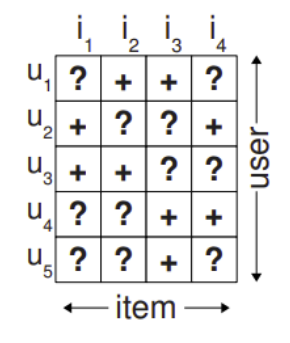
\includegraphics[width=\textwidth]{images/implicit.png}
					
					{\tiny Source: \textit{BPR: Bayesian Personalized Ranking from Implicit Feedback}, Rendle et al. 2012}
				\end{center}
			\end{column}
		\end{columns}
	\end{frame}

	\begin{frame}
		\frametitle{How to get $u_i$ and $v_j$}
		\begin{itemize}
			\item The score function: $u_i^\top v_j$ \pause
			\item Matrix Factorization: where user and item representations are static and independent of each other (fixing the model). \pause
			\item RNN To integrate user history, $u_i = f(v_{u, 1}, v_{u, 2}, \cdots, v_{u, n})$
			\begin{itemize}
				\item The user representation now depends on his/her previously interacted items. \pause
			\end{itemize}
			\item Graph-based models to integrate neighboring items/users (in the next slide).
			\begin{itemize}
				\item The user representation could also depend on behaviors of other users/items.  \pause
			\end{itemize}
			\item Can combine with content-based recommendation (i.e. with user and item features). \pause
			\item Scoring function can also change (e.g. to bilinear $u_i^\top Q v_j$)
		\end{itemize}
	\end{frame}

	\begin{frame}
		\frametitle{\only<1-5>{GCMC: Learning $u_i$ and $v_j$ from User-Item Graph}\only<6>{Simplifying GCMC to GraphSAGE}}
		\begin{center}
			\centering
			\includegraphics[width=0.5\textwidth]{images/bipartite.png}
			
			{\tiny Source: \textit{Graph Convolutional Matrix Completion}, van den Berg et al. 2017}
		\end{center}
		\begin{enumerate}
			\item $\mu_{v_j \to u_i, r} = \frac{1}{c_{u_i v_j}} \only<1-5>{W_r}\only<6>{\alert{W}} x_{v_j}$ \pause
			\item $h_{u_i} = \sigma \left[\mathrm{agg}\left(
		\sum_{v_j \in \only<1-5>{\mathcal{N}_{u_i,1}}\only<6>{\alert{\mathcal{S}(\mathcal{N}_{u_i,1})}}} \mu_{v_j \to u_i, 1},
		\cdots,
		\sum_{v_j \in \only<1-5>{\mathcal{N}_{u_i,R}}\only<6>{\alert{\mathcal{S}(\mathcal{N}_{u_i,R})}}} \mu_{v_j \to u_i, R}
		\right) \right]$ \pause
			\item $u_i = \sigma(W_u h_{u_i})$ and similarly we compute $v_j$ \pause
			\item \only<1-5>{$p(\hat{M}_{ij}=r) = \mathrm{softmax}(u_i^\top Q_r v_j)$}%
			\only<6>{\alert{$r_{i,j} = u_i^\top v_j$} to predict rating} \pause
			\item When new interactions are added, just re-run the forward pass on the new graph to get new $u_i$ and $v_j$.
		\end{enumerate}
	\end{frame}

	\begin{frame}
		\frametitle{Learning $u_i$ and $v_j$ with Star-GCN}
		\begin{center}
			\centering
			\includegraphics[width=\textwidth]{images/stargcn.png}
		\end{center}
		\begin{itemize}
			\item Vanilla GCMC can't deal with new users/items without features (but with a few interactions).
			\item STAR-GCN
			\begin{itemize}
				\item "Mask" the user/item embedding to 0 as if it is new.
				\item Reconstruct the embedding after the forward pass and reconstruction pass.
			\end{itemize}
		\end{itemize}
	\end{frame}

	\begin{frame}
		\frametitle{Learning $v_j$ and $u_i$ from Item-Item and User-User Graph}
		\begin{columns}
			\begin{column}{0.6\textwidth}
				\begin{itemize}
					\item<1-> Decompose the user-item graph into user-user graph and item-item graph.
					\item<2-> Get $u_i$ with a Graph Convolutional Network on user-user graph and $v_j$ on item-item graph.
					\item<3-> Compute $r_{i,j} = u_i^\top v_j$
					\item<4-> $u_i$ and $v_j$ can be learned with
					\begin{itemize}
						\item Direct neighbor sampling (GraphSAGE)
						\item Random-walk based neighbor sampling (PinSAGE)
					\end{itemize}
					\item<5-> When new interactions are added, just re-run the forward pass on the new graph to get new $u_i$ and $v_j$.
				\end{itemize}
			\end{column}
			\begin{column}{0.4\textwidth}<1->
				\begin{center}
					\centering
					\includegraphics[width=\textwidth]{images/decompose.png}
				\end{center}
			\end{column}
		\end{columns}
	\end{frame}

	\begin{frame}
		\frametitle{Other Meaningful Aspects to Consider}
		\begin{itemize}
			\item \textbf{Cold-start}: What if we have \textit{new} users and items coming in, with few to no historical interactions? \pause
			\item \textbf{Bias correction}: The training dataset usually comes from the result of a \textit{previous recommender system}.  How to mitigate the bias? \pause
			\item \textbf{Diversity}: Always recommending the same items (or even the same kind of item) to a user would make him/her feel \textit{bored}. \pause
			\item \textbf{Fraud}: How to detect and deal with fabricated explicit feedbacks (e.g. fake ratings and reviews)?
		\end{itemize}
	\end{frame}

	\begin{frame}
		\begin{center}
			\centering
			\Huge Coding Session
			
			\Large GraphSAGE on bipartite user-item graph.
		\end{center}
	\end{frame}
\end{document}